\section{Grundlagen} \label{sec:Grundlagen}

\subsection{Software-Qualitätsmetriken} \label{sec:SoftwareQualitaetsmetriken}
%Hier muss ich noch was zu den metrikern schreiben, was sind software qualitätsmetriken, was sind die eigenschaften, was sind die anforderungen an software qualitätsmetriken, wann kamen sie auf



Qualitätsmetriken sind Kennzahlen, die zur Bewertung der Qualität verwendet werden. Sie sind ein wichtiges Werkzeug zur Analyse und Verbesserung jeglicher Dinge. Im grunde sind metriken einfach nur messungen, die eine bestimmte Aussagekraft haben. OFt ist es nicht möglich eine Metrik zu identifizieren, die eine vollumfängliche aussage über etwas trifft. Oft ist es notwenig verschiedene metriken im zusammenspiel miteinander zu betrachten, um ein verständis für aspekte zu erhalten. 

Dies gilt auch für Software-Qualitätsmetriken: \enquote{Eine Softwarequalitätsmetrik ist eine Funktion, die eine Software-Einheit in einen Zahlenwert abbildet, welcher als Erfüllungsgrad einer Qualitätseigenschaft der Software-Einheit interpretierbar ist.}\cite{def_qual_metric}

Es ist nicht möglich eine einzige Metrik zu finden, die eine vollumfängliche aussage über die Qualität einer Software trifft - was ist schon gute Software? Wann ist software gut? SEblst wenn man als Ziel von software definieren würde, dass sie fehlerfrei ist, wäre es nicht möglich eine einzige Metrik zu finden, die dies beschreibt. Wann ist eine software fehlerfrei? Ist sie fehlerfrei, wenn sie keine Bugs hat? Wenn sie keine Bugs hat, aber trotzdem nicht benutzbar ist, ist sie dann fehlerfrei?

Dieser Eigenschaft macht es notwendig verschiedene Metriken im zusammenspiel zu betrachten und sich einen übersblick über die Indizien zu verschaffen, die auf eine gute oder schlechte Qualität hinweisen.
Die besonderheit bei Software-Qualitätsmetriken im vergleich zu anderen Metriken mag sein, dass die Daten hierarchisch strukturiert sind. Meist wird dies auf die orderner und datei-struktur abgebildet. So werden die Metriken in der Regel auf der Ebene der einzelnen Dateien ermittelt und dann auf die Ordner-Ebene aggregiert, wodurch eine hierarchische Baumstruktur entsteht. 

Software-Qualitätsmetriken werden meist auf Software-Einheiten angewendet. Also z.B. auf Dateien des Quellcodes, auf Module oder auf Klassen. Diese Software-Einheiten sind in der Regel hierarchisch strukturiert. Auch die im folgenden vorgesllten ansätze zur Visualisierung von hierarchischen Daten sind nicht speziell für Software-Qualitätsmetriken gedacht, sondern stellen allgemeine Ansätze dar. Ich behaupte, dass die Sturktur von Software gemeinsamkeiten hat, zB. ein ordner hat nicht mehr als 20 Kinder, was interessante annahmen darstellt, die eventuell in die visualierungs algorithmen verbessernd einfließen können.  

\subsection{Treemap-Layouts} \label{sec:Treemap}

Eine Treemap visualisiert einen Baum, indem jedem Knoten ein Rechteck mit der Fläche A zugewiesen wird, proportional zu seinem zugewiesenen Wert (z.B. Datenmenge oder Marktwert). Nicht-Blatt-Knoten werden dabei üblicherweise durch Rahmen (Container-Rectangles) gekennzeichnet, um die Gruppierung der Kinder zu zeigen. \cite{bruls2000squarified} Die Rechtecke aller Blätter füllen die Fläche des Wurzelrechtecks vollständig aus. Mathematisch entspricht die Eingabedatenstruktur einem gewichteten Baum, bei dem jede Blatteinheit eine numerische Größe hat. Die Fläche eines Eltern-Rechtecks entspricht der Summe der Flächen (Werte) seiner Kinder.

Die konkrete Idee hierarchische DAten in form von Treemaps darzustellen wurde erstmals 1991 von Shneiderman und Johnson \cite{johnson1991tree} vorgestellt. Sie stellten fest, dass die Darstellung von hierarchischen Daten in Form von Bäumen in der Regel nicht sehr anschaulich ist. Sie entwickelten eine Methode, um diese Daten in Form von Rechtecken darzustellen, die die Fläche der Knoten proportional zu ihrem Wert darstellen. Diese Methode wurde als \enquote{Treemap} bezeichnet. Als Ziele dieser Visualierung formulierten sie unter anderem diese Aspekte:
\begin{itemize}
    \item \textbf{Effiziente Nutzung des Platzes:} Generell soll es darum gehen möglichst viele Informationen auf einem kleinen Raum darzustellen.
    \item \textbf{Verständlichkeit:} Die Visualisierung soll so gestaltet sein, dass sie für den Betrachter leicht verständlich ist. Es soll möglich sein schnell und mit nur niedrigem kognitiven Aufwand die dargesllten Informationen zu erfassen.
    \item \textbf{Ästethik:} Die Visualisierung soll ansprechend gestaltet sein.
\end{itemize}

Zuvor bestehende Ansätze zur Visualisierung von hierarchischen Daten waren in der Regel nicht sehr anschaulich, besonders, wenn es um große Datenmengen ging. Listen, Baumdiagramme (siehe Abbildung \) oder andere Darstellungen (auch bekannt als Node oder Link-Diagramme) sind nicht in der lage alle diese Aspekte zu erfüllen. Bei Einem typischen Baumdiagram zum Beispiel werden teilweise mehr als die Hälfte der Fläche für Hintergrund genutzt \cite[3]{johnson1991tree} außerdem ist es schwer, außer der Struktur der Daten auch die Metriken darzustellen. Sie kritisieren auch die Darstellung von hierarchischen Daten in Form von Venn-Diagrammen (siehe Abbildung \ref{fig:venndiagram}): \enquote{The space required between regions would certainly preclude this Venn diagram representation from serious consideration for larger structures.}\cite[5]{johnson1991tree} Es ist zwar möglich durch die Größe der Kreise eine Metrik darzustellen, es sei aber nicht möglich eine große Anzahl an Knoten sinnvoll darzustellen. 

\begin{figure}[H]
    \centering
    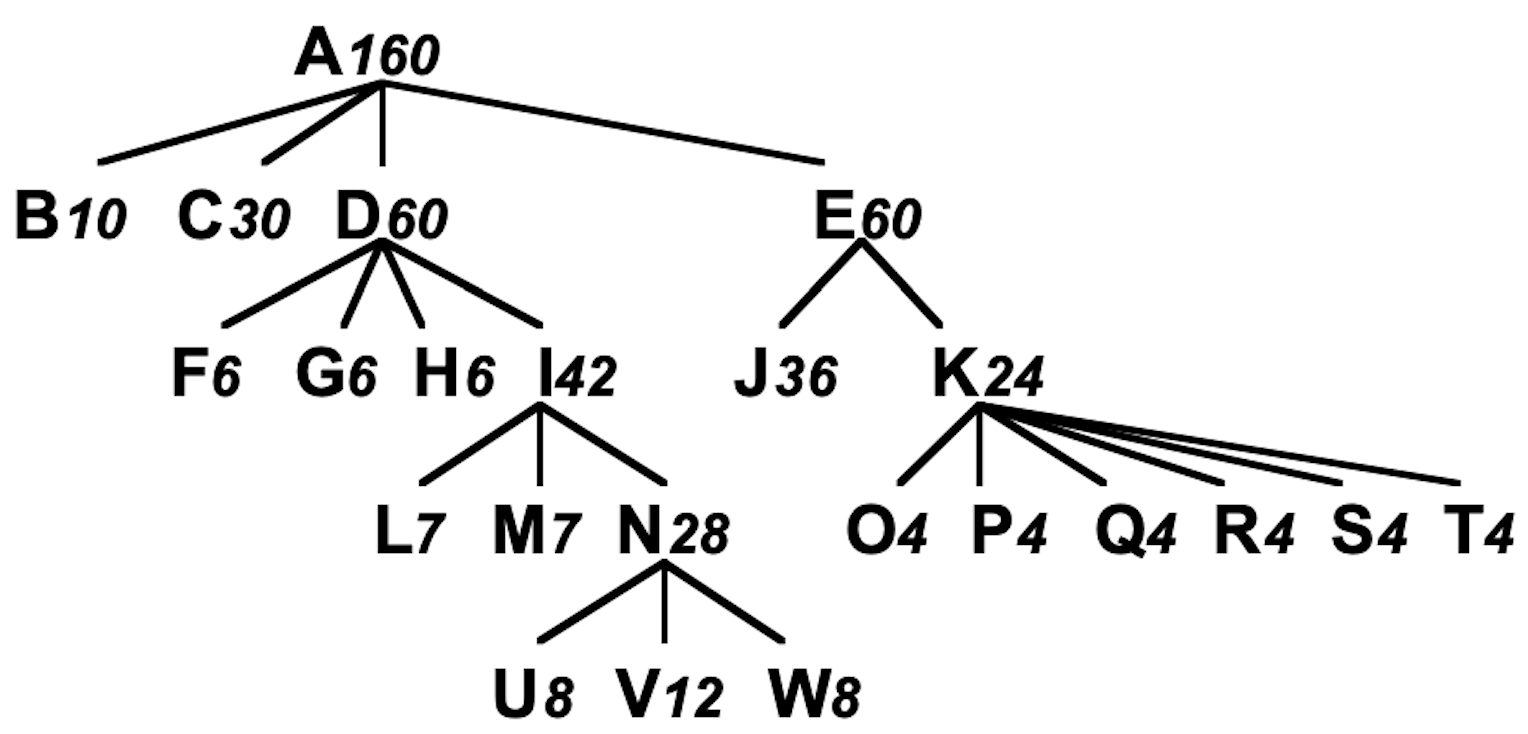
\includegraphics[width=0.5\textwidth]{images/treediagram.png}
    \caption{Beispiel für ein Baumdiagramm}
    \label{fig:baumdiagramm}
\end{figure}

\begin{figure}[H]
    \centering
    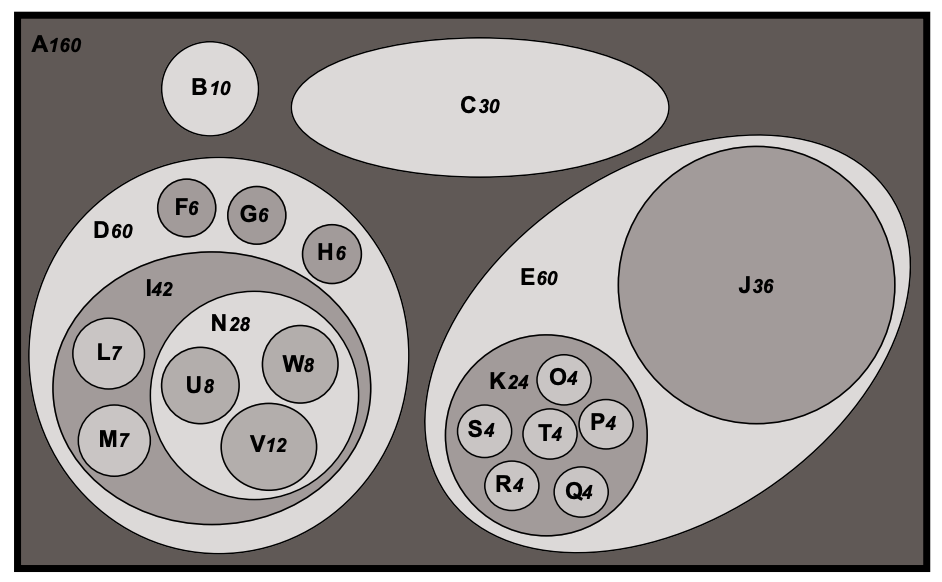
\includegraphics[width=0.5\textwidth]{images/verdiagram.png}
    \caption{Beispiel für ein Venn-Diagramm}
    \label{fig:venndiagram}
\end{figure}

\enquote{Using boxes instead of ovals and a bin-packing algorithm could partially solve this space
problem. But bin-packing is an NP-complete problem and does not preserve order.}\cite[5]{johnson1991tree} Sie stellen fest, dass es theoretisch eine dem Venn Diagramm ähnliche Lösung gibt, die allerdings NP-Hard ist. 

\begin{figure}[H]
    \centering
    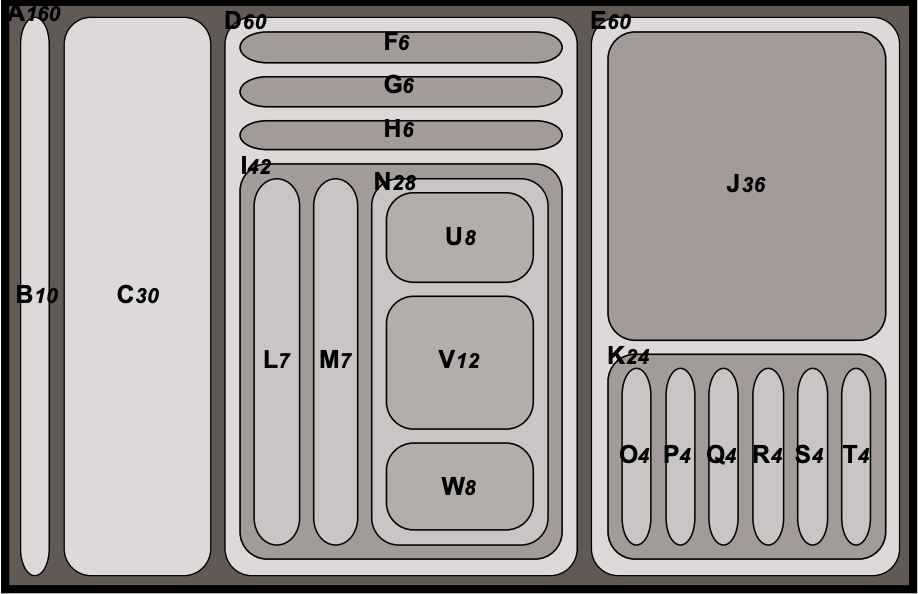
\includegraphics[width=0.5\textwidth]{images/rectVennDiagram.png}
    \caption{Beispiel für ein Boxed Venn-Diagramm}
    \label{fig:rectVennDiagramm}
\end{figure}

Shneiderman und Johnson schlagen zur Lösung dieser Schwierigkeiten ihren Treemap ansatz vor. Sie legen vier Eigenschaften fest, die bei der Erstellung der Treemaps gewährleistet werden:

\begin{itemize}
    \item Wenn ein Knoten 1 ein Vorfahre von Knoten 2 ist, dann ist der Bereich von Knoten 1 vollständig enthalten in dem Bereich von Knoten 2.
    \item Die Bereiche von zwei Knoten schneiden sich, wenn ein Knoten ein Vorfahre des anderen ist.
    \item Knoten belegen eine Fläche, die streng proportional zu ihrem Gewicht ist.
    \item Das Gewicht eines Knotens ist größer oder gleich der Summe der Gewichte seiner Kinder.
\end{itemize}

Sie stellen auch einen Algorithmus vor, der diese Eigenschaften erfüllen soll. Ein von diesem Algorithmus erzeugtes Layout ist in Abbildung \ref{fig:nestedTreemap} dargestellt. 

\begin{figure}[H]
    \centering
    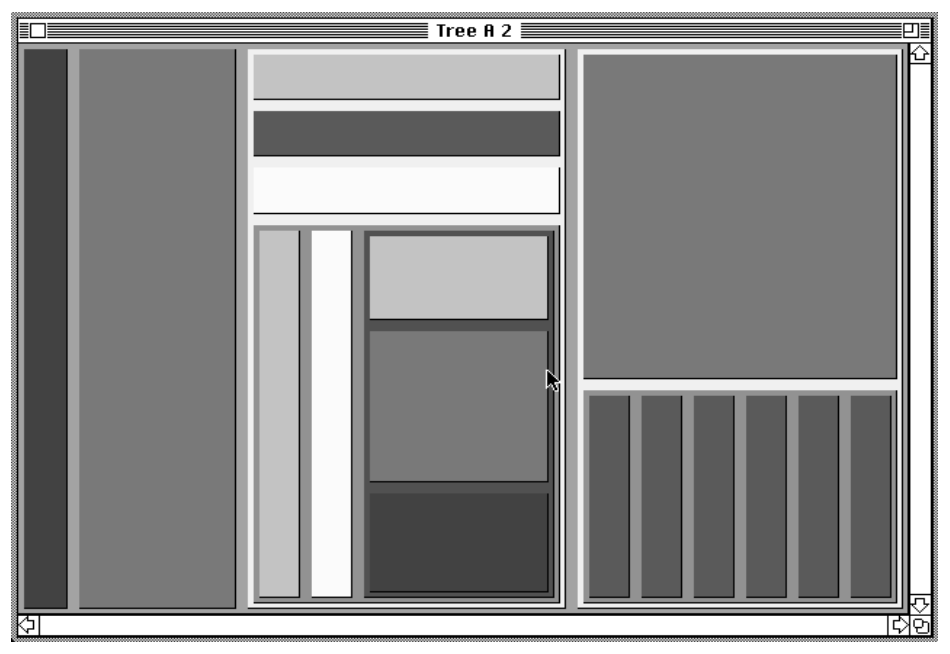
\includegraphics[width=0.5\textwidth]{images/nestedTreemapDiagramm.png}
    \caption{Beispiel für eine Treemap}
    \label{fig:nestedTreemap}
\end{figure}

Der Algorithmus unterteilt den Raum abwechselnd vertikal und horizontal, je nach größe der Knoten. Der Algorithmus arbeitet sich rekursiv von der Wurzel bis zu den Blättern herunter und hat eine Laufzeit von O(n), wobei n die Anzahl der Knoten ist. Im nächsten Abschnitt wird ein ähnlicher Algorithmus im Detail beschrieben, was zum besseren verständis dieser Art von Algorithmen helfen wird.

Obwohl es sich hier um ein renomiertes und viel Zitiertes Paper handelt, machen die Authoren einen entscheidenden Fehler, der in manchen Fällen sogar dazu führen kann, dass Rechtecke komplett verschwinden. Die Authoren betrachten dieses Problem in ihrem Paper leider nicht. 
Der Abstand zwischen den Knoten wird nämlich dadurch erzeugt, dass die Rechtecke diesen Abstand links, recht, oben und unten abgezogen bekommen. Dadurch ist die dargestellte Fläche der Rechtecke nicht mehr proportional zu den Werten, die sie darstellen sollen. Eigenschaft 3 wird also verletzt. Dies ist besonders problematisch, wenn die Rechtecke sehr klein bzw. sehr langgezogen sind. In diesem Fall kann es dazu kommen, dass die Rechtecke so klein werden, dass sie nicht mehr dargestellt werden können. Dies stellt in der Praxis ein riesiges Problem dar, speziell wenn das Problem dieser Arbeit also 3D im kopf bahalten wird. Es kann ja theoretisch vorkommen, dass als Flächenmetrik die lines of code verwendet wird und dort ein file, weil er wenige lines hat sehr klein wird und deswegen aufgrund der margins nicht angezeigt wird. Wenn jetzt aber die metrik für die Höhen berechnung die prozentualle test abdeckung der lines ist und der file nicht getestet ist, dann würde ein potentiell großes problem, was auch eigentlich direkt in auge springen sollte, nicht angezeigt werden. 

Ein weiteres Problem bei diesem Algorithmus ist auch generell, dass unter umständen die Rechtecke sehr langgezogen werden können, was unter Umständen auch Kriterium 3 der Ästethik verletzt. Es gibt viele Ideen dieses Problem anzugehen. Eine Möglichkeit, den Squarify Algorithmus zu verwenden, wird im nöchsten Abschnitt vorgestellt.

\subsubsection{Squarify-Algorithmus} \label{sec:Squarify}

Der Squarify-Algorithmus ist ein Layout-Algorithmus für Treemaps, der darauf abzielt, die Fläche der Rechtecke so ausgewogen wie möglich zu gestalten. Beduetet, dass die Rechtecke möglichst quadratisch sind. Die ursprüngliche form des algorithmusses wurde im Jahr 2000 von Bruls et al. \cite{bruls2000squarified} vorgestellt. Sie stellten fest: \enquote{another problem of standard treemaps [is] the emergence of thin, elongated rectangles}\cite[1]{bruls2000squarified}. wenn rechtecke nicht mehr so langgezogen sind, Es ist einfacher auf Rechtecke zu zeigen, diese wahrzunehmen, sie zu vergleichen und ihre größe einzuschätzen. 

Der Algorithmus arbeitet rekursiv und teilt die Fläche in Rechtecke auf, wobei er versucht, die Seitenverhältnisse der Rechtecke so nah wie möglich an 1 zu halten. Sie stellen einen Rekursiven ansatz vor, die so wie auch die meisten anderen treemap algorithmen von top to bottom (also vom root knoten bis zu den blatt knoten) die rechtecke aufgeteilt werden.  

Im folgenden wird der Algorithmus beschrieben, da er eine wichtige Grundlage für das verständis des Problems darstellt und außerdem eine gute Grundlage zum verständis der anderen Algorithmen darstellt, da viele Algorithmen ähnliche Ideen verwenden.

Der Algorithmus wird an folgendem Beispiel aus dem original Squarify-Paper \cite[5]{bruls2000squarified} erleutert. Wir werden den Algorithmus selbst aber anders erklären als in dem Paper, da wir uns näher an der implementierungen, wie sie in der bekannten d3 bibliothek \cite{d3_treemap_code} umgesetzt ist halten.
Es sollen Rechtecke mit den Größen 6, 6, 4, 3, 2, 2, 1 in ein 6 mal 4 Recheck einsortiert werden.

Der algorithmus arbeitet immer in Reihen, die er versucht zu füllen und dabei die Rechtecke möglichst quadratisch zu halten. Das erste Rechteck ist breiter als lang. (In dieser Arbeit werden wir, anders als in den herkömmlichen papern zu layout algorithmen, das Wort breit als x koordinate und das wort lang als y koordinate nutzen - das hat den hintergrund, dass das wort hoch im drei dimensionalen meist für die z komponent genutzt wird und es sonst zu verwirrungen kommen könnte)
Da das Rechteck in das wir einfügen breiter als lang ist, werden wir eine imaginäre horizontale Reihe so lange mit Rechtecken befüllen, bis ein Threshold erreicht ist. Das erste Rechteck mit größe 6 fügen wir also in Schritt 1 in diese Reihe ein. Das Seitenverhältnis dieses Rechtecks beträgt 8 zu 3 (das Rechteck ist 1.5 Einheiten breit und 4 Einheiten lang). Das zweite Rechteck mit größe 6 fügen wir in Schritt 2 in diese horizontale Reihe ein, dabei wird die Reihe entsprechend breiter. Das Seitenverhältnis des jetzt eingefügten Rechecks beträgt 3 zu 2 (das Rechteck ist 3 Einheiten breit und 2 Einheiten lang). Jetzt kommt das nächste Rechteck mit größe 4. Dieses Rechteck ist hat ein Seitenverhältnis von 4 zu 1 (das Rechteck ist 4 Einheiten breit und 1 Einheit lang).   



Das Ziel ist es das Verhältnis der Seitenlängen gleich zu halten. Im ursprünglichen Paper von Bruls et al. \cite{bruls2000squarified} wird darauf noch nicht so eingegangen, aber viele implementierungen z.b. die von d3.js \cite{d3_treemap_code} ermöglichen es, das Verhältnis nicht nur an den Wert 1 anzunähern, sondern auch an andere Werte, zum Beispiel den goldenen Schnitt. 
%hier vllt ein vergleichs bild einfügen






